\chapter{Data Encryption in Linux Systems}
\label{chapter:enc-linux}

This chapter explains more detailed the concept of encryption and presents the handling of data encryption in traditional (non-Android) Linux systems.

\section{Encryption explained}
\label{sec:enc-explained}

%http://library.ahima.org/xpedio/groups/public/documents/ahima/bok1_048923.hcsp?dDocName=bok1_048923
Encryption is a mathematical transformation which scrambles data requiring protection (plaintext) into a form not easily understood by unauthorized entities (ciphertext). After being transformed into ciphertext, the plaintext appears random and does not reveal anything about the content of the original data.

Encryption is a reversible transformation. This reversal process is referred to as decryption. An encryption process has a corresponding decryption process, which is used to reverse the encrypted data (ciphertext) back to its original content (plaintext).

Each encryption and decryption function requires a cryptographic key. A cryptographic key is a string of binary digits used as an input to encryption and decryption functions.

\begin{figure}[h]
\centering
\begin{minipage}{0.45\textwidth}
\centering
  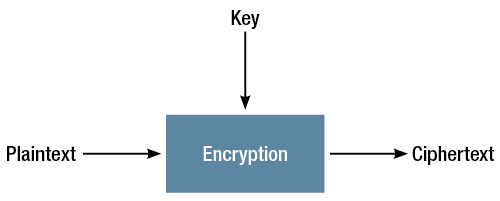
\includegraphics[width=.9\linewidth]{src/img/encrypt/plain2cypher.jpg}
  \caption{Encryption}
  \label{fig:encrypt-fig}
\end{minipage}\hfill
\begin{minipage}{0.45\textwidth}
\centering
  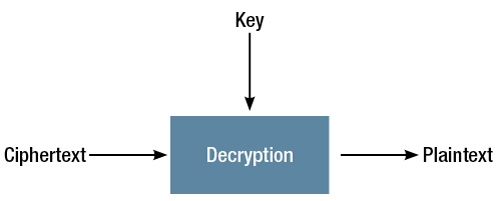
\includegraphics[width=.9\linewidth]{src/img/encrypt/cypher2plain.jpg}
  \caption{Decrpytion}
  \label{fig:decrypt-fig}
\end{minipage}
\end{figure}

For the purposes of disk encryption, each blockdevice (or individual file in the case of stacked filesystem encryption) is divided into sectors of equal length, for example 512 bytes (4,096 bits). The encryption/decryption then happens on a per-sector basis, so the n'th sector of the blockdevice/file on disk will store the encrypted version of the n'th sector of the original data.

Whenever the operating system or an application requests a certain fragment of data from the blockdevice/file, the whole sector (or sectors) that contains the data will be read from disk, decrypted on-the-fly, and temporarily stored in memory:

Similarly, on each write operation, all sectors that are affected must be re-encrypted complelety (while the rest of the sectors remain untouched).

In order to be able to de/encrypt data, the disk encryption system needs to know the unique secret key associated with it. Whenever the encrypted block device or folder in question is to be mounted, its corresponding key (called henceforth its \textit{master key}) must be supplied.

The following are some of the possible methods of storing and cryptographically securing a master key with a keyfile:
\begin{enumerate}
\item \textbf{Stored in a plaintext keyfile}

Simply storing the master key in a file (in readable form) is the simplest option. The file, called a \textit{keyfile}, can be placed on a removable device that is only connected to the computer when mounting the encrypted parts of the disk.

\item \textbf{Randomly generated on-the-fly for each session}

In some cases, e.g. when encrypting swap space or a /tmp partition, it is not necessary to keep a persistent master key at all. A new throwaway key can be randomly generated for each session, without requiring any user interaction. This means that once unmounted, all files written to the partition in question can never be decrypted again by anyone - which in those particular use-cases is perfectly fine.

\item \textbf{Stored in passphrase-protected form in a keyfile or on the disk itself}

The master key (and thus the encrypted data) can be protected with a secret passphrase, which you will have to remember and enter each time you want to mount the encrypted block device or folder.
It is usually not used for de/encrypting the disk data directly, though. For example, in the case of stacked filesystem encryption, each file can be automatically assigned its own encryption key. Whenever the file is to be read/modified, this file key first needs to be decrypted using the main key, before it can itself be used to de/encrypt the file contents.

\end{enumerate}

\subsection{Benefits of disk encryption}
\label{sub-sec:benefits-enc}

Disk encryption is the process of storing data on disk in an encrypted form. The files only become available to the operating system and applications in readable form while the system is running and unlocked with the corresponding key.

Disk encryption methods aim to provide three distinct properties:
\begin{enumerate}
\item The data on the disk should remain confidential
\item Read and write operations should both be fast, regardless of where on the disk the data is stored
\item The overhead introduced by the encryption method should not be kept to a minimum (i.e., the amount of storage used for encrypted data should not be significantly larger than the size of plaintext)
\end{enumerate}

Disk encryption can prevent unauthorized viewing of the data when the computer or hard-disk is:
\begin{itemize}
\item located in a place to which non-trusted people might gain access while you are away
\item lost or stolen, as with laptops, netbooks or external storage devices
\item in the repair shop
\item discarded after its end-of-life
\end{itemize}

The system will still be vulnerable to:
\begin{itemize}
\item Attackers who can break into the system (e.g. over the Internet) while it is running and after the encrypted parts of the disk have already been unlocked and mounted.
\item Attackers who are able to gain physical access to the computer while it is running (even if you use a screenlocker), or very shortly after it was running, if they have the resources to perform a cold boot attack.
\item A government entity which may obtain your keys/passphrases using various techniques of coercion. It may be legal for law enforcement agencies to do so if they have suspicions that you might be hiding something of interest.
\end{itemize}

\subsection{Data Encryption vs System Encryption}
\label{sub-sec:de-vs-se}

\textbf{Data encryption} is defined as encrypting only the user's data itself (often located within the /home directory). While it is the simplest and least intrusive use of disk encryption, it has some significant drawbacks.
In modern computing systems, there are many background processes that may cache/store information about user data or parts of the data itself in non-encrypted areas of the hard drive, like:
\begin{itemize}
\item swap partitions
\item /tmp (temporary files created by user applications)
\item /var (log files and databases)
\end{itemize}


\textbf{System encryption} is the encryption of the operating system and user data, which helps to address some of the inadequacies of data encryption.

Benefits:
\begin{itemize}
\item prevents unauthorized physical access to operating system files
\item prevents unauthorized physical access to private data that may be cached by the system
\end{itemize}
Disadvantages:
\begin{itemize}
\item unlocking of the encrypted parts of the disk can no longer happen during or after user login; it must now happen at boot time
\end{itemize}
In practice, there is not always a clear line between data encryption and system encryption.

Finally, it is important that disk encryption be viewed as an adjunct to the existing security mechanisms of the operating system, while relying on other parts of the system to provide things like network security and user-based access control.

\subsection{Block Encryption vs Stacked File System Encryption}
\label{sub-sec:be-vs-sfse}

The two approaches to disk encryption are block-based and file-based. Block encryption means that the actual encryption process happens when the filesystem writes a block of data on the disk. Its advantages are simplicity and transparency. However, the method lacks granularity, i.e., treating each file differently. This is the type of encryption used in Android 3.0 and later.

A more in detail comparison of block-based encryption and file-based encryption is presented in the following table.\footnote{\url{http://ksouedu.com/doc/ecryptfs-utils/ecryptfs-faq.html\#compare}}

\renewcommand{\arraystretch}{1.8}
\begin{center}
\begin{table}[tp]
	\begin{tabularx}{\textwidth}{|| m{0.46\textwidth} || m{0.46\textwidth} ||}
		\hhline{|t:=:t:=:t|}
		\multicolumn{1}{||c||}{\textbf{Block Device Encryption}} & 
			\multicolumn{1}{c||}{\textbf{Stacked Filesystem Encryption}} \\ 
		\hhline{|:=::=:|}
		Simple in concept and implementation; just transform blocks as they pass through. & High level of design complexity; meticulous handling of internal filesystem primitives required. \\
		\hhline{|:=::=:|}
		Must allocate a block device to dedicate for the entire filesystem. & Stacks on top of existing mounted filesystems; requires no special on-disk storage allocation effort. \\
		\hhline{|:=::=:|}
		Everything in the filesystem incurs the cost of encryption and decryption, regardless of the confidentiality requirements for the data. & Selective encryption of the contents of only the sensitive files. \\
		\hhline{|:=::=:|}
		Fully protects the confidentiality of the directory structures, superblocks, file sizes, file permissions, and so forth. & Cannot keep all filesystem metadata confidential. Since stacked filesystems encrypt on a per-file basis, attackers will know the approximate file sizes, for instance. \\
		\hhline{|:=::=:|}
		Coarse granularity; only fixed per-mountpoint encryption policies are possible. & Fine granularity; flexible per-file encryption policies are possible. \\
		\hhline{|:=::=:|}		
		No notion of ``encrypted files.'' Individual files must be re-encrypted via a userspace application before written to backups, sent via email, etc. & Individual encrypted files can be accessed transparently by applications; no additional work needed on the part of applications before moving the files to another location. \\
		\hhline{|:=::=:|}
		Clients cannot use directly on networked filesystems; encryption must be set up and managed on the server, or the client must encase all of his files in a loopback mount, losing the per-file granularity from the perspective of other clients. & Clients can stack on locally mounted networked filesystems; individual files are sent to the server and stored in encrypted form. \\
		\hhline{|:=::=:|}
		Can protect databases that use their own dedicated block device. & Can only protect databases that write their tables to regular files in an existing filesystem. \\
		\hhline{|:=::=:|}
		Used to protect swap space. & Not designed to protect swap space; we recommend using block device encryption to protect swap space while using eCryptfs on the filesystem. \\
		\hhline{|:=::=:|}
		Possible to hide the fact that the partition is encrypted. & The fact that encrypted data exists on the device is obvious to an observer. \\
		\hhline{|:=::=:|}
		Filesystem-agnostic; any filesystem will work on an encrypted block device. & Can only be expected to work with existing filesystems that are upstream in the official Linux kernel. \\
		\hhline{|b:=:b:=:b|}
	\end{tabularx}
	\caption{Block Device Encryption vs Stacked Filesystem Encryption}
\end{table}
\end{center}
\newpage

\section{eCryptfs}
\label{sec:de-ecryptfs}

As mentioned before, eCryptfs is a stacked file system which manages data encryption. Now, details about it and the advantages and disadvantages is brings will be presented.

Originally authored by Michael Halcrow and the IBM LInux Technology Center, eCryptfs is derived from Erez Zadok's Cryptfs, and the FiST framework for stacked filesystems. eCryptfs extended Cryptfs to provide advanced key management and policy features. 
